% Options for packages loaded elsewhere
\PassOptionsToPackage{unicode}{hyperref}
\PassOptionsToPackage{hyphens}{url}
\PassOptionsToPackage{dvipsnames,svgnames,x11names}{xcolor}
%
\documentclass[
  letterpaper,
  DIV=11,
  numbers=noendperiod]{scrartcl}

\usepackage{amsmath,amssymb}
\usepackage{iftex}
\ifPDFTeX
  \usepackage[T1]{fontenc}
  \usepackage[utf8]{inputenc}
  \usepackage{textcomp} % provide euro and other symbols
\else % if luatex or xetex
  \usepackage{unicode-math}
  \defaultfontfeatures{Scale=MatchLowercase}
  \defaultfontfeatures[\rmfamily]{Ligatures=TeX,Scale=1}
\fi
\usepackage{lmodern}
\ifPDFTeX\else  
    % xetex/luatex font selection
\fi
% Use upquote if available, for straight quotes in verbatim environments
\IfFileExists{upquote.sty}{\usepackage{upquote}}{}
\IfFileExists{microtype.sty}{% use microtype if available
  \usepackage[]{microtype}
  \UseMicrotypeSet[protrusion]{basicmath} % disable protrusion for tt fonts
}{}
\makeatletter
\@ifundefined{KOMAClassName}{% if non-KOMA class
  \IfFileExists{parskip.sty}{%
    \usepackage{parskip}
  }{% else
    \setlength{\parindent}{0pt}
    \setlength{\parskip}{6pt plus 2pt minus 1pt}}
}{% if KOMA class
  \KOMAoptions{parskip=half}}
\makeatother
\usepackage{xcolor}
\setlength{\emergencystretch}{3em} % prevent overfull lines
\setcounter{secnumdepth}{-\maxdimen} % remove section numbering
% Make \paragraph and \subparagraph free-standing
\ifx\paragraph\undefined\else
  \let\oldparagraph\paragraph
  \renewcommand{\paragraph}[1]{\oldparagraph{#1}\mbox{}}
\fi
\ifx\subparagraph\undefined\else
  \let\oldsubparagraph\subparagraph
  \renewcommand{\subparagraph}[1]{\oldsubparagraph{#1}\mbox{}}
\fi

\usepackage{color}
\usepackage{fancyvrb}
\newcommand{\VerbBar}{|}
\newcommand{\VERB}{\Verb[commandchars=\\\{\}]}
\DefineVerbatimEnvironment{Highlighting}{Verbatim}{commandchars=\\\{\}}
% Add ',fontsize=\small' for more characters per line
\usepackage{framed}
\definecolor{shadecolor}{RGB}{241,243,245}
\newenvironment{Shaded}{\begin{snugshade}}{\end{snugshade}}
\newcommand{\AlertTok}[1]{\textcolor[rgb]{0.68,0.00,0.00}{#1}}
\newcommand{\AnnotationTok}[1]{\textcolor[rgb]{0.37,0.37,0.37}{#1}}
\newcommand{\AttributeTok}[1]{\textcolor[rgb]{0.40,0.45,0.13}{#1}}
\newcommand{\BaseNTok}[1]{\textcolor[rgb]{0.68,0.00,0.00}{#1}}
\newcommand{\BuiltInTok}[1]{\textcolor[rgb]{0.00,0.23,0.31}{#1}}
\newcommand{\CharTok}[1]{\textcolor[rgb]{0.13,0.47,0.30}{#1}}
\newcommand{\CommentTok}[1]{\textcolor[rgb]{0.37,0.37,0.37}{#1}}
\newcommand{\CommentVarTok}[1]{\textcolor[rgb]{0.37,0.37,0.37}{\textit{#1}}}
\newcommand{\ConstantTok}[1]{\textcolor[rgb]{0.56,0.35,0.01}{#1}}
\newcommand{\ControlFlowTok}[1]{\textcolor[rgb]{0.00,0.23,0.31}{#1}}
\newcommand{\DataTypeTok}[1]{\textcolor[rgb]{0.68,0.00,0.00}{#1}}
\newcommand{\DecValTok}[1]{\textcolor[rgb]{0.68,0.00,0.00}{#1}}
\newcommand{\DocumentationTok}[1]{\textcolor[rgb]{0.37,0.37,0.37}{\textit{#1}}}
\newcommand{\ErrorTok}[1]{\textcolor[rgb]{0.68,0.00,0.00}{#1}}
\newcommand{\ExtensionTok}[1]{\textcolor[rgb]{0.00,0.23,0.31}{#1}}
\newcommand{\FloatTok}[1]{\textcolor[rgb]{0.68,0.00,0.00}{#1}}
\newcommand{\FunctionTok}[1]{\textcolor[rgb]{0.28,0.35,0.67}{#1}}
\newcommand{\ImportTok}[1]{\textcolor[rgb]{0.00,0.46,0.62}{#1}}
\newcommand{\InformationTok}[1]{\textcolor[rgb]{0.37,0.37,0.37}{#1}}
\newcommand{\KeywordTok}[1]{\textcolor[rgb]{0.00,0.23,0.31}{#1}}
\newcommand{\NormalTok}[1]{\textcolor[rgb]{0.00,0.23,0.31}{#1}}
\newcommand{\OperatorTok}[1]{\textcolor[rgb]{0.37,0.37,0.37}{#1}}
\newcommand{\OtherTok}[1]{\textcolor[rgb]{0.00,0.23,0.31}{#1}}
\newcommand{\PreprocessorTok}[1]{\textcolor[rgb]{0.68,0.00,0.00}{#1}}
\newcommand{\RegionMarkerTok}[1]{\textcolor[rgb]{0.00,0.23,0.31}{#1}}
\newcommand{\SpecialCharTok}[1]{\textcolor[rgb]{0.37,0.37,0.37}{#1}}
\newcommand{\SpecialStringTok}[1]{\textcolor[rgb]{0.13,0.47,0.30}{#1}}
\newcommand{\StringTok}[1]{\textcolor[rgb]{0.13,0.47,0.30}{#1}}
\newcommand{\VariableTok}[1]{\textcolor[rgb]{0.07,0.07,0.07}{#1}}
\newcommand{\VerbatimStringTok}[1]{\textcolor[rgb]{0.13,0.47,0.30}{#1}}
\newcommand{\WarningTok}[1]{\textcolor[rgb]{0.37,0.37,0.37}{\textit{#1}}}

\providecommand{\tightlist}{%
  \setlength{\itemsep}{0pt}\setlength{\parskip}{0pt}}\usepackage{longtable,booktabs,array}
\usepackage{calc} % for calculating minipage widths
% Correct order of tables after \paragraph or \subparagraph
\usepackage{etoolbox}
\makeatletter
\patchcmd\longtable{\par}{\if@noskipsec\mbox{}\fi\par}{}{}
\makeatother
% Allow footnotes in longtable head/foot
\IfFileExists{footnotehyper.sty}{\usepackage{footnotehyper}}{\usepackage{footnote}}
\makesavenoteenv{longtable}
\usepackage{graphicx}
\makeatletter
\def\maxwidth{\ifdim\Gin@nat@width>\linewidth\linewidth\else\Gin@nat@width\fi}
\def\maxheight{\ifdim\Gin@nat@height>\textheight\textheight\else\Gin@nat@height\fi}
\makeatother
% Scale images if necessary, so that they will not overflow the page
% margins by default, and it is still possible to overwrite the defaults
% using explicit options in \includegraphics[width, height, ...]{}
\setkeys{Gin}{width=\maxwidth,height=\maxheight,keepaspectratio}
% Set default figure placement to htbp
\makeatletter
\def\fps@figure{htbp}
\makeatother

\usepackage{booktabs}
\usepackage{longtable}
\usepackage{array}
\usepackage{multirow}
\usepackage{wrapfig}
\usepackage{float}
\usepackage{colortbl}
\usepackage{pdflscape}
\usepackage{tabu}
\usepackage{threeparttable}
\usepackage{threeparttablex}
\usepackage[normalem]{ulem}
\usepackage{makecell}
\usepackage{xcolor}
\KOMAoption{captions}{tableheading}
\makeatletter
\makeatother
\makeatletter
\makeatother
\makeatletter
\@ifpackageloaded{caption}{}{\usepackage{caption}}
\AtBeginDocument{%
\ifdefined\contentsname
  \renewcommand*\contentsname{Table of contents}
\else
  \newcommand\contentsname{Table of contents}
\fi
\ifdefined\listfigurename
  \renewcommand*\listfigurename{List of Figures}
\else
  \newcommand\listfigurename{List of Figures}
\fi
\ifdefined\listtablename
  \renewcommand*\listtablename{List of Tables}
\else
  \newcommand\listtablename{List of Tables}
\fi
\ifdefined\figurename
  \renewcommand*\figurename{Figure}
\else
  \newcommand\figurename{Figure}
\fi
\ifdefined\tablename
  \renewcommand*\tablename{Table}
\else
  \newcommand\tablename{Table}
\fi
}
\@ifpackageloaded{float}{}{\usepackage{float}}
\floatstyle{ruled}
\@ifundefined{c@chapter}{\newfloat{codelisting}{h}{lop}}{\newfloat{codelisting}{h}{lop}[chapter]}
\floatname{codelisting}{Listing}
\newcommand*\listoflistings{\listof{codelisting}{List of Listings}}
\makeatother
\makeatletter
\@ifpackageloaded{caption}{}{\usepackage{caption}}
\@ifpackageloaded{subcaption}{}{\usepackage{subcaption}}
\makeatother
\makeatletter
\@ifpackageloaded{tcolorbox}{}{\usepackage[skins,breakable]{tcolorbox}}
\makeatother
\makeatletter
\@ifundefined{shadecolor}{\definecolor{shadecolor}{rgb}{.97, .97, .97}}
\makeatother
\makeatletter
\makeatother
\makeatletter
\makeatother
\ifLuaTeX
  \usepackage{selnolig}  % disable illegal ligatures
\fi
\IfFileExists{bookmark.sty}{\usepackage{bookmark}}{\usepackage{hyperref}}
\IfFileExists{xurl.sty}{\usepackage{xurl}}{} % add URL line breaks if available
\urlstyle{same} % disable monospaced font for URLs
\hypersetup{
  colorlinks=true,
  linkcolor={blue},
  filecolor={Maroon},
  citecolor={Blue},
  urlcolor={Blue},
  pdfcreator={LaTeX via pandoc}}

\author{}
\date{}

\begin{document}
\ifdefined\Shaded\renewenvironment{Shaded}{\begin{tcolorbox}[boxrule=0pt, breakable, sharp corners, interior hidden, borderline west={3pt}{0pt}{shadecolor}, enhanced, frame hidden]}{\end{tcolorbox}}\fi

\hypertarget{segunda-entrega---pruxe1ctico-2}{%
\section{Segunda entrega - Práctico
2}\label{segunda-entrega---pruxe1ctico-2}}

\hypertarget{ejercicio-5}{%
\subsection{EJERCICIO 5}\label{ejercicio-5}}

\textbf{Suponga que en una aplicación económica donde se quiere modelar
el ahorro de un conjunto de hogares en función de sus ingresos, el
modelo correcto a aplicar es:}
\(ahorro_i = \beta_0 + \beta_1 \, ingreso_i + \epsilon_i\) \textbf{Pero
usted, decide eliminar la constante del modelo debido a que sin ingresos
es imposible ahorrar. Por ende, ajusta el siguiente modelo:}
\(ahorro_i = \beta_1^{*} \, ingreso_i + \epsilon_i^{*}\)

\textbf{1. Demuestre que el estimador de mınimos cuadrados es:}
\(\hat{\beta}_1 = \frac{\sum_i ingreso_i \cdot ahorro_i}{\sum_i ingreso_i^2}\)

\(\hat{\beta}_{\text{MCO}} = (X^{\top} X)^{-1} X^{\top} Y\)

Para el modelo reducido tenemos que \(x_i = ingreso_i\) e
\(y_i =ahorro_i\)

\(X= \begin{pmatrix}ingreso_1 \\ingreso_2 \\\vdots \\ingreso_n\end{pmatrix}\)
\(Y=\begin{pmatrix}ahorro_1 \\ahorro_2 \\\vdots \\ahorro_n\end{pmatrix}\)

\(X^{\top} X = (ingreso_1, ingreso_2, \ldots, ingreso_n)\begin{pmatrix} ingreso_1 \\ ingreso_2 \\ \vdots \\ ingreso_n\end{pmatrix}= \sum_{i=1}^n ingreso_i^2\)

\((X^{\top} X) ^{-1} = \left( \sum_{i=1}^n ingreso_i ^2 \right) ^{-1} = \frac{1}{\sum_{i=1}^n ingreso_i^2}\)

\(X^{\top} Y = (ingreso_1, ingreso_2, \ldots, ingreso_n)\begin{pmatrix}ahorro_1 \\ahorro_2 \\\vdots \\ahorro_n\end{pmatrix}= \sum_{i=1}^n ingreso_i \, ahorro_i\)

\(\Rightarrow \hat{\beta}_{\text{MCO}} = \hat{\beta^{*}}_{1} = \frac{\sum_{i=1}^n ingreso_i \, ahorro_i}{\sum_{i=1}^n ingreso_i^2}\)

\textbf{2. Demuestre que (si el modelo correcto incluye la constante)
este estimador es sesgado.}

Siguiendo la ppt de la clase 6 (diapositiva 14) se define para
\(Y = X_1 \beta_1 + X_2 \beta_2 + \epsilon\)

\(E\left(\hat{\beta}_1^{*}\right)= \beta_1 + (X_1^{\top} X_1)^{-1} X_1^{\top} X_2 \beta_2\)

La esperanza de \(\beta_1\) para el modelo reducido, omitiendo
\(\beta_2 X_2\)

En nuestro caso

\(Y=\begin{pmatrix}ahorro_1 \\ahorro_2 \\\vdots \\ahorro_n\end{pmatrix}\)
\(X_1= \begin{pmatrix}ingreso_1 \\ingreso_2 \\\vdots \\ingreso_n\end{pmatrix}\)

y \(X_2 = \begin{pmatrix}1 \\1 \\\vdots \\1\end{pmatrix}\) una constante
omitida pero relevante con \(\beta_2 = \beta_0\)

\((X_1 ^{\top} X_1) ^{-1} = \frac{1}{\sum_{i=1}^n ingreso_i ^2}\)

\(X_1^{\top} X_2=(ingreso_1, ingreso_2, \ldots, ingreso_n)\begin{pmatrix}1 \\1 \\\vdots \\1\end{pmatrix}= \sum_{i=1}^n ingreso_i\)

\(E\left(\hat{\beta}_1^{*}\right)= \beta_1 + \frac{\sum_{i=1}^n ingreso_i}{\sum_{i=1}^n ingreso_i^2} \, \beta_0\)

Asumimos que \(\beta_0 \neq 0\)

\(\Rightarrow\) SESGADO

\textbf{3. Encuentre una expresión para dicho sesgo.}

(Notas Inferencia p.72) Definición 3.4.2.

Para un estimador real \(T\) de \(\tau(\theta)\) , el sesgo de \(T\) se
define como
\(B_{\theta}(T) = E_{\theta}(T) - \tau(\theta), \theta \in \Theta\).

En nuestro caso, usando la definición tenemos que:
\(B(\hat{\beta}_1^{*}) = E(\hat{\beta}_1 ^{ * } ) - \beta_1\)

Sustituyendo:

\(B(\hat{\beta}_1^{*}) = \left( \beta_1 + \frac{\sum_{i=1}^n ingreso_i}{\sum_{i=1}^n ingreso_i^2} \, \beta_0 \right) - \beta_1 \Rightarrow B(\hat{\beta}_1^{*}) = \frac{\sum_{i=1}^n ingreso_i}{\sum_{i=1}^n ingreso_i^2} \, \beta_0\)

\textbf{4. ¿Qué idea se le ocurre para solucionar el problema del sesgo
y continuar trabajando con el modelo sin constante?}

Centar las variables seria buena idea para eliminar el sesgo sin incluir
explicitamente la constante. Al hacer esto, pasan a tener media 0, que
implica que la variable explicativa es ortogonal a la constante.
Graficamente veriamos que la recta ajustada pasa por el origen (0),
preservando la pendiente.

Sea \(\tilde{X_1}=X_1 - E(X_1)\). Queremos estudiar su ortogonalidad
respecto a \(X_2\)

\(\tilde{X}_1 \perp X_2 \;\Longleftrightarrow\; \langle X_1, X_2 \rangle = 0\)

Ademas sabemos que por propiedad la media es el punto de equilibrio.
Entonces

\(\tilde{x}_i = x_i - \bar{x}\quad \Rightarrow \quad\sum_{i=1}^n \tilde{x}_i = 0\)

\(\langle \tilde{X_1}, X_2 \rangle = \tilde{X}_1^\top X_2 = (\tilde{ingreso}_1, \tilde{ingreso}_2, \ldots, \tilde{ingreso}_n)\begin{pmatrix}1 \\ 1 \\ \vdots \\ 1\end{pmatrix}= \sum_{i=1}^n \tilde{ingreso}_i = 0\)

Entonces son ortogonales

\hypertarget{ejercicio-7}{%
\subsection{EJERCICIO 7}\label{ejercicio-7}}

\textbf{En el archivo pgc.txt se encuentran las mediciones de 252
personas. Se desea construir una fórmula que sea capaz de estimar el
porcentaje de grasa corporal en función de algunas mediciones
(circunferencia abdominal, circunferencia de cintura, de cuello, entre
otras).}

\begin{Shaded}
\begin{Highlighting}[]
\CommentTok{\#cargo librerias}
\FunctionTok{library}\NormalTok{(tidyverse)}
\end{Highlighting}
\end{Shaded}

\begin{verbatim}
-- Attaching core tidyverse packages ------------------------ tidyverse 2.0.0 --
v dplyr     1.1.4     v readr     2.1.5
v forcats   1.0.0     v stringr   1.5.1
v ggplot2   3.5.2     v tibble    3.2.1
v lubridate 1.9.3     v tidyr     1.3.1
v purrr     1.0.4     
-- Conflicts ------------------------------------------ tidyverse_conflicts() --
x dplyr::filter() masks stats::filter()
x dplyr::lag()    masks stats::lag()
i Use the conflicted package (<http://conflicted.r-lib.org/>) to force all conflicts to become errors
\end{verbatim}

\begin{Shaded}
\begin{Highlighting}[]
\FunctionTok{library}\NormalTok{(ggcorrplot)}
\FunctionTok{library}\NormalTok{(kableExtra) }\CommentTok{\#no hace falta la verdad}
\end{Highlighting}
\end{Shaded}

\begin{verbatim}

Attaching package: 'kableExtra'

The following object is masked from 'package:dplyr':

    group_rows
\end{verbatim}

\begin{Shaded}
\begin{Highlighting}[]
\FunctionTok{library}\NormalTok{(knitr)}
\CommentTok{\#otras librerias alternativas {-}{-}\textgreater{} GGally para usar ggpairs}

\NormalTok{data }\OtherTok{\textless{}{-}} \FunctionTok{read.table}\NormalTok{(}\StringTok{"pgc.txt"}\NormalTok{, }\AttributeTok{header =} \ConstantTok{TRUE}\NormalTok{, }\AttributeTok{dec =} \StringTok{","}\NormalTok{) }
\CommentTok{\#guardo data organizada, fue medio un desastre al principio}

\FunctionTok{str}\NormalTok{(data) }\CommentTok{\#ver la clase de las variables}
\end{Highlighting}
\end{Shaded}

\begin{verbatim}
'data.frame':   252 obs. of  14 variables:
 $ porc_grasa: num  12.6 6.9 24.6 10.9 27.8 20.6 19 12.8 5.1 12 ...
 $ edad      : int  23 22 22 26 24 24 26 25 25 23 ...
 $ peso      : num  70 78.6 69.9 83.8 83.6 95.4 82.1 79.8 86.6 89.9 ...
 $ altura    : num  166 177 162 177 175 ...
 $ cuello    : num  36.2 38.5 34 37.4 34.4 39 36.4 37.8 38.1 42.1 ...
 $ pecho     : num  93.1 93.6 95.8 101.8 97.3 ...
 $ abdomen   : num  85.2 83 87.9 86.4 100 94.4 90.7 88.5 82.5 88.6 ...
 $ cadera    : num  94.5 98.7 99.2 101.2 101.9 ...
 $ muslo     : num  59 58.7 59.6 60.1 63.2 66 58.4 60 62.9 63.1 ...
 $ rodilla   : num  37.3 37.3 38.9 37.3 42.2 42 38.3 39.4 38.3 41.7 ...
 $ tobillo   : num  21.9 23.4 24 22.8 24 25.6 22.9 23.2 23.8 25 ...
 $ biceps    : num  32 30.5 28.8 32.4 32.2 35.7 31.9 30.5 35.9 35.6 ...
 $ brazo     : num  27.4 28.9 25.2 29.4 27.7 30.6 27.8 29 31.1 30 ...
 $ muneca    : num  17.1 18.2 16.6 18.2 17.7 18.8 17.7 18.8 18.2 19.2 ...
\end{verbatim}

\begin{Shaded}
\begin{Highlighting}[]
\NormalTok{data[] }\OtherTok{\textless{}{-}} \FunctionTok{sapply}\NormalTok{(data, as.numeric) }\CommentTok{\#lo paso a numericos}
\end{Highlighting}
\end{Shaded}

\textbf{1. Visualice la relación de cada una de las medidas corporales
con respecto a la variable porc\_grasa y estime las correlaciones.}

\begin{Shaded}
\begin{Highlighting}[]
\NormalTok{data\_long }\OtherTok{\textless{}{-}} \FunctionTok{pivot\_longer}\NormalTok{(data, }\AttributeTok{cols =} \SpecialCharTok{{-}}\NormalTok{porc\_grasa)}

\FunctionTok{ggplot}\NormalTok{(data\_long, }\FunctionTok{aes}\NormalTok{(}\AttributeTok{x =}\NormalTok{ value, }\AttributeTok{y =}\NormalTok{ porc\_grasa)) }\SpecialCharTok{+}
  \FunctionTok{geom\_point}\NormalTok{(}\AttributeTok{color =} \StringTok{"violet"}\NormalTok{, }\AttributeTok{alpha =} \FloatTok{0.8}\NormalTok{) }\SpecialCharTok{+}
  \FunctionTok{geom\_smooth}\NormalTok{(}\AttributeTok{method =} \StringTok{"lm"}\NormalTok{, }\AttributeTok{se =} \ConstantTok{FALSE}\NormalTok{, }\AttributeTok{color =} \StringTok{"deeppink"}\NormalTok{) }\SpecialCharTok{+}
  \FunctionTok{facet\_wrap}\NormalTok{(}\SpecialCharTok{\textasciitilde{}}\NormalTok{name, }\AttributeTok{scales =} \StringTok{"free\_x"}\NormalTok{) }\SpecialCharTok{+}
  \FunctionTok{theme\_minimal}\NormalTok{() }
\end{Highlighting}
\end{Shaded}

\begin{verbatim}
`geom_smooth()` using formula = 'y ~ x'
\end{verbatim}

\begin{figure}[H]

{\centering 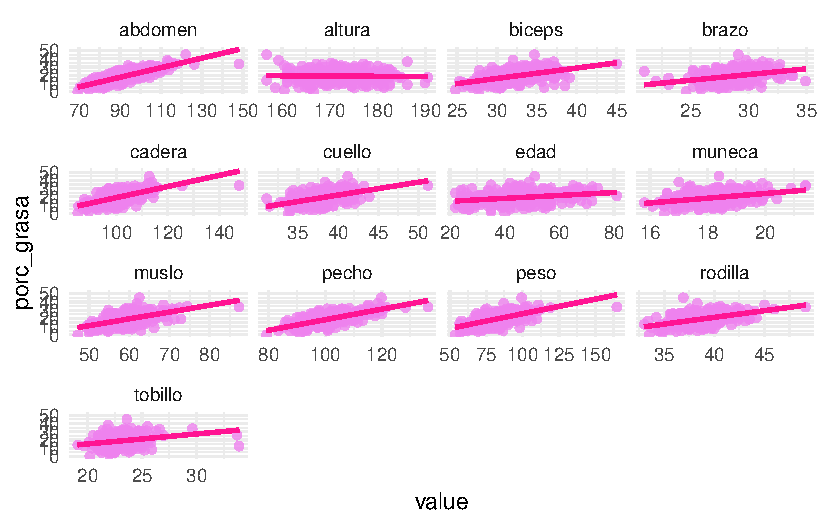
\includegraphics{entrega2_files/figure-pdf/unnamed-chunk-2-1.pdf}

}

\end{figure}

\begin{Shaded}
\begin{Highlighting}[]
\FunctionTok{kable}\NormalTok{(}\FunctionTok{cor}\NormalTok{(data}\SpecialCharTok{$}\NormalTok{porc\_grasa, data[ , }\FunctionTok{names}\NormalTok{(data) }\SpecialCharTok{!=} \StringTok{"porc\_grasa"}\NormalTok{]))}
\end{Highlighting}
\end{Shaded}

\begin{longtable}[]{@{}
  >{\raggedleft\arraybackslash}p{(\columnwidth - 24\tabcolsep) * \real{0.0763}}
  >{\raggedleft\arraybackslash}p{(\columnwidth - 24\tabcolsep) * \real{0.0763}}
  >{\raggedleft\arraybackslash}p{(\columnwidth - 24\tabcolsep) * \real{0.0840}}
  >{\raggedleft\arraybackslash}p{(\columnwidth - 24\tabcolsep) * \real{0.0763}}
  >{\raggedleft\arraybackslash}p{(\columnwidth - 24\tabcolsep) * \real{0.0763}}
  >{\raggedleft\arraybackslash}p{(\columnwidth - 24\tabcolsep) * \real{0.0763}}
  >{\raggedleft\arraybackslash}p{(\columnwidth - 24\tabcolsep) * \real{0.0763}}
  >{\raggedleft\arraybackslash}p{(\columnwidth - 24\tabcolsep) * \real{0.0763}}
  >{\raggedleft\arraybackslash}p{(\columnwidth - 24\tabcolsep) * \real{0.0763}}
  >{\raggedleft\arraybackslash}p{(\columnwidth - 24\tabcolsep) * \real{0.0763}}
  >{\raggedleft\arraybackslash}p{(\columnwidth - 24\tabcolsep) * \real{0.0763}}
  >{\raggedleft\arraybackslash}p{(\columnwidth - 24\tabcolsep) * \real{0.0763}}
  >{\raggedleft\arraybackslash}p{(\columnwidth - 24\tabcolsep) * \real{0.0763}}@{}}
\toprule\noalign{}
\begin{minipage}[b]{\linewidth}\raggedleft
edad
\end{minipage} & \begin{minipage}[b]{\linewidth}\raggedleft
peso
\end{minipage} & \begin{minipage}[b]{\linewidth}\raggedleft
altura
\end{minipage} & \begin{minipage}[b]{\linewidth}\raggedleft
cuello
\end{minipage} & \begin{minipage}[b]{\linewidth}\raggedleft
pecho
\end{minipage} & \begin{minipage}[b]{\linewidth}\raggedleft
abdomen
\end{minipage} & \begin{minipage}[b]{\linewidth}\raggedleft
cadera
\end{minipage} & \begin{minipage}[b]{\linewidth}\raggedleft
muslo
\end{minipage} & \begin{minipage}[b]{\linewidth}\raggedleft
rodilla
\end{minipage} & \begin{minipage}[b]{\linewidth}\raggedleft
tobillo
\end{minipage} & \begin{minipage}[b]{\linewidth}\raggedleft
biceps
\end{minipage} & \begin{minipage}[b]{\linewidth}\raggedleft
brazo
\end{minipage} & \begin{minipage}[b]{\linewidth}\raggedleft
muneca
\end{minipage} \\
\midrule\noalign{}
\endhead
\bottomrule\noalign{}
\endlastfoot
0.2891735 & 0.6132242 & -0.0224272 & 0.4914889 & 0.7028852 & 0.8137062 &
0.6256999 & 0.5612844 & 0.5077859 & 0.2667826 & 0.4930309 & 0.3632774 &
0.3475728 \\
\end{longtable}

\begin{Shaded}
\begin{Highlighting}[]
\CommentTok{\#redundate con la matriz de correlacion}
\end{Highlighting}
\end{Shaded}

\begin{enumerate}
\def\labelenumi{\arabic{enumi}.}
\setcounter{enumi}{1}
\tightlist
\item
  \textbf{Estime la matriz de correlación de las mediciones corporales}
\end{enumerate}

\begin{Shaded}
\begin{Highlighting}[]
\NormalTok{mdecor }\OtherTok{\textless{}{-}} \FunctionTok{cor}\NormalTok{(data) }\CommentTok{\#devuelve varianza y correlaciones de la variables, es decir la matriz}

\FunctionTok{kable}\NormalTok{(mdecor)}
\end{Highlighting}
\end{Shaded}

\begin{longtable}[]{@{}
  >{\raggedright\arraybackslash}p{(\columnwidth - 28\tabcolsep) * \real{0.0688}}
  >{\raggedleft\arraybackslash}p{(\columnwidth - 28\tabcolsep) * \real{0.0688}}
  >{\raggedleft\arraybackslash}p{(\columnwidth - 28\tabcolsep) * \real{0.0688}}
  >{\raggedleft\arraybackslash}p{(\columnwidth - 28\tabcolsep) * \real{0.0688}}
  >{\raggedleft\arraybackslash}p{(\columnwidth - 28\tabcolsep) * \real{0.0688}}
  >{\raggedleft\arraybackslash}p{(\columnwidth - 28\tabcolsep) * \real{0.0625}}
  >{\raggedleft\arraybackslash}p{(\columnwidth - 28\tabcolsep) * \real{0.0625}}
  >{\raggedleft\arraybackslash}p{(\columnwidth - 28\tabcolsep) * \real{0.0625}}
  >{\raggedleft\arraybackslash}p{(\columnwidth - 28\tabcolsep) * \real{0.0688}}
  >{\raggedleft\arraybackslash}p{(\columnwidth - 28\tabcolsep) * \real{0.0688}}
  >{\raggedleft\arraybackslash}p{(\columnwidth - 28\tabcolsep) * \real{0.0625}}
  >{\raggedleft\arraybackslash}p{(\columnwidth - 28\tabcolsep) * \real{0.0688}}
  >{\raggedleft\arraybackslash}p{(\columnwidth - 28\tabcolsep) * \real{0.0688}}
  >{\raggedleft\arraybackslash}p{(\columnwidth - 28\tabcolsep) * \real{0.0688}}
  >{\raggedleft\arraybackslash}p{(\columnwidth - 28\tabcolsep) * \real{0.0625}}@{}}
\toprule\noalign{}
\begin{minipage}[b]{\linewidth}\raggedright
\end{minipage} & \begin{minipage}[b]{\linewidth}\raggedleft
porc\_grasa
\end{minipage} & \begin{minipage}[b]{\linewidth}\raggedleft
edad
\end{minipage} & \begin{minipage}[b]{\linewidth}\raggedleft
peso
\end{minipage} & \begin{minipage}[b]{\linewidth}\raggedleft
altura
\end{minipage} & \begin{minipage}[b]{\linewidth}\raggedleft
cuello
\end{minipage} & \begin{minipage}[b]{\linewidth}\raggedleft
pecho
\end{minipage} & \begin{minipage}[b]{\linewidth}\raggedleft
abdomen
\end{minipage} & \begin{minipage}[b]{\linewidth}\raggedleft
cadera
\end{minipage} & \begin{minipage}[b]{\linewidth}\raggedleft
muslo
\end{minipage} & \begin{minipage}[b]{\linewidth}\raggedleft
rodilla
\end{minipage} & \begin{minipage}[b]{\linewidth}\raggedleft
tobillo
\end{minipage} & \begin{minipage}[b]{\linewidth}\raggedleft
biceps
\end{minipage} & \begin{minipage}[b]{\linewidth}\raggedleft
brazo
\end{minipage} & \begin{minipage}[b]{\linewidth}\raggedleft
muneca
\end{minipage} \\
\midrule\noalign{}
\endhead
\bottomrule\noalign{}
\endlastfoot
porc\_grasa & 1.0000000 & 0.2891735 & 0.6132242 & -0.0224272 & 0.4914889
& 0.7028852 & 0.8137062 & 0.6256999 & 0.5612844 & 0.5077859 & 0.2667826
& 0.4930309 & 0.3632774 & 0.3475728 \\
edad & 0.2891735 & 1.0000000 & -0.0126788 & -0.2455175 & 0.1135052 &
0.1764497 & 0.2304094 & -0.0503321 & -0.2000958 & 0.0175157 & -0.1050581
& -0.0411621 & -0.0850556 & 0.2135306 \\
peso & 0.6132242 & -0.0126788 & 1.0000000 & 0.4879517 & 0.8307019 &
0.8941979 & 0.8879807 & 0.9408611 & 0.8686880 & 0.8531476 & 0.6137599 &
0.8005109 & 0.6301386 & 0.7297720 \\
altura & -0.0224272 & -0.2455175 & 0.4879517 & 1.0000000 & 0.3202702 &
0.2274898 & 0.1910599 & 0.3748292 & 0.3412596 & 0.5024881 & 0.3934893 &
0.3189629 & 0.3216992 & 0.3965094 \\
cuello & 0.4914889 & 0.1135052 & 0.8307019 & 0.3202702 & 1.0000000 &
0.7848350 & 0.7540774 & 0.7349579 & 0.6956973 & 0.6724050 & 0.4778924 &
0.7311459 & 0.6236603 & 0.7448264 \\
pecho & 0.7028852 & 0.1764497 & 0.8941979 & 0.2274898 & 0.7848350 &
1.0000000 & 0.9158277 & 0.8294199 & 0.7298586 & 0.7194964 & 0.4829879 &
0.7279075 & 0.5801727 & 0.6601623 \\
abdomen & 0.8137062 & 0.2304094 & 0.8879807 & 0.1910599 & 0.7540774 &
0.9158277 & 1.0000000 & 0.8740662 & 0.7666239 & 0.7371789 & 0.4532227 &
0.6849827 & 0.5033161 & 0.6198324 \\
cadera & 0.6256999 & -0.0503321 & 0.9408611 & 0.3748292 & 0.7349579 &
0.8294199 & 0.8740662 & 1.0000000 & 0.8964098 & 0.8234726 & 0.5583868 &
0.7392725 & 0.5450141 & 0.6300895 \\
muslo & 0.5612844 & -0.2000958 & 0.8686880 & 0.3412596 & 0.6956973 &
0.7298586 & 0.7666239 & 0.8964098 & 1.0000000 & 0.7991703 & 0.5397971 &
0.7614774 & 0.5668422 & 0.5586848 \\
rodilla & 0.5077859 & 0.0175157 & 0.8531476 & 0.5024881 & 0.6724050 &
0.7194964 & 0.7371789 & 0.8234726 & 0.7991703 & 1.0000000 & 0.6116082 &
0.6787088 & 0.5558982 & 0.6645073 \\
tobillo & 0.2667826 & -0.1050581 & 0.6137599 & 0.3934893 & 0.4778924 &
0.4829879 & 0.4532227 & 0.5583868 & 0.5397971 & 0.6116082 & 1.0000000 &
0.4848545 & 0.4190500 & 0.5661946 \\
biceps & 0.4930309 & -0.0411621 & 0.8005109 & 0.3189629 & 0.7311459 &
0.7279075 & 0.6849827 & 0.7392725 & 0.7614774 & 0.6787088 & 0.4848545 &
1.0000000 & 0.6782551 & 0.6321264 \\
brazo & 0.3632774 & -0.0850556 & 0.6301386 & 0.3216992 & 0.6236603 &
0.5801727 & 0.5033161 & 0.5450141 & 0.5668422 & 0.5558982 & 0.4190500 &
0.6782551 & 1.0000000 & 0.5855883 \\
muneca & 0.3475728 & 0.2135306 & 0.7297720 & 0.3965094 & 0.7448264 &
0.6601623 & 0.6198324 & 0.6300895 & 0.5586848 & 0.6645073 & 0.5661946 &
0.6321264 & 0.5855883 & 1.0000000 \\
\end{longtable}

\begin{Shaded}
\begin{Highlighting}[]
\CommentTok{\#visualizar}
\FunctionTok{ggcorrplot}\NormalTok{(}\FunctionTok{cor}\NormalTok{(data)) }\CommentTok{\#mapa de calor de matriz de correlacion}
\end{Highlighting}
\end{Shaded}

\begin{figure}[H]

{\centering 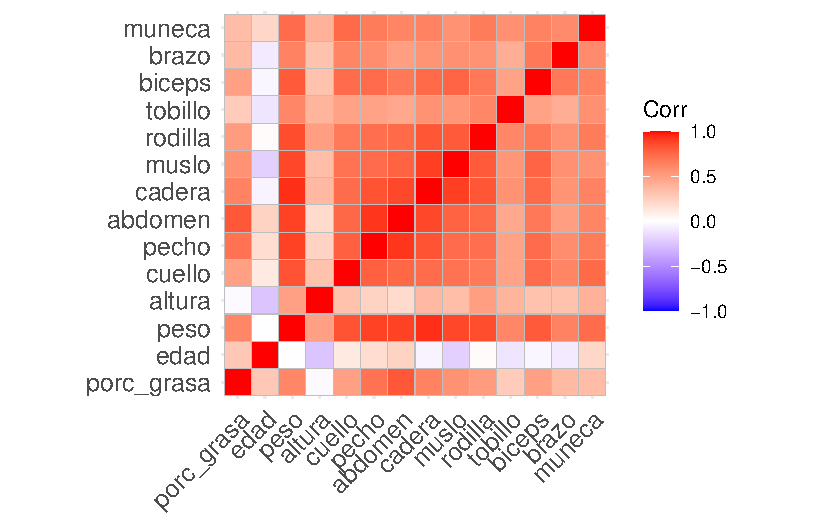
\includegraphics{entrega2_files/figure-pdf/unnamed-chunk-3-1.pdf}

}

\end{figure}

\begin{enumerate}
\def\labelenumi{\arabic{enumi}.}
\setcounter{enumi}{2}
\tightlist
\item
  \textbf{Describa con sus palabras las conclusiones que haya podido
  obtener a partir de los dos puntos anteriores.}
\end{enumerate}

En el gráfico de dispersión se puede observar una relación positiva
entre porc\_grasa y la mayoría de las variables, aunque en algunos casos
más marcado que otros. Por ejemplo, se observa que la variable abdomen y
cadera estan fuertemente relacionadas, presentando (en la recta ajustado
por ggplot con el método lm, linear model) una pendiente mayor respecto
a altura y edad. En estas últimas dos variables se observa una pendiente
casi nula.

En el mapa de calor de la matriz de correlación se corrobora esta
afirmación. Altura y edad tienen un coeficiente de correlación respecto
a porcentaje grasa en un color mas intenso cercano a 1, mientras que la
altura por ejemplo es muy parecido a blanco (0). Los valores exactos los
obtenemos en la matriz de correlación, los cuales sustentan las ideas de
los gráficos. Abdomen tiene una correlación con el porcentaje de grasa
de un 0.8, cadera 0.6. , y edad 0.28. Por otro lado, altura -0.02.

Se presencia el vínculo entre la pendiente de la recta de RLS y el
coeficiente de correlación lineal, permitiendo determinar fuerza y
sentido de la relación y comparten el mismo signo. No obstante, el
segundo esta normalizado entre -1 y 1, mientras que la pendiente depende
de las unidades de medida

\begin{enumerate}
\def\labelenumi{\arabic{enumi}.}
\setcounter{enumi}{3}
\tightlist
\item
  \textbf{Realice un conjunto de modelos de RLS (regresión lineal
  simple) que expliquen la relacion de cada medida corporal con respecto
  al porcentaje de grasa corporal. ¿Qué observa?}
\end{enumerate}

\begin{Shaded}
\begin{Highlighting}[]
\NormalTok{explicativas }\OtherTok{\textless{}{-}} \FunctionTok{names}\NormalTok{(data)[}\FunctionTok{names}\NormalTok{(data) }\SpecialCharTok{!=} \StringTok{"porc\_grasa"}\NormalTok{]}
\CommentTok{\#sacar los nombres de la variables explicativas}

\NormalTok{modelitos }\OtherTok{\textless{}{-}} \FunctionTok{lapply}\NormalTok{(explicativas, }
      \ControlFlowTok{function}\NormalTok{(x)\{ }\CommentTok{\#ajustar modelo para cada una}
        \FunctionTok{lm}\NormalTok{(}\FunctionTok{as.formula}\NormalTok{(}\FunctionTok{paste}\NormalTok{(}\StringTok{"porc\_grasa \textasciitilde{}"}\NormalTok{, x)), }\AttributeTok{data =}\NormalTok{ data)}
\NormalTok{      \})}

\CommentTok{\#ahora queremos ver la info/summary de cada uno}
\NormalTok{resumencitos }\OtherTok{\textless{}{-}} \FunctionTok{lapply}\NormalTok{(modelitos, summary)}
\FunctionTok{names}\NormalTok{(resumencitos) }\OtherTok{\textless{}{-}}\NormalTok{ explicativas}

\NormalTok{resumencitos}
\end{Highlighting}
\end{Shaded}

\begin{verbatim}
$edad

Call:
lm(formula = as.formula(paste("porc_grasa ~", x)), data = data)

Residuals:
     Min       1Q   Median       3Q      Max 
-18.0697  -5.7025   0.2846   4.8301  25.0739 

Coefficients:
            Estimate Std. Error t value Pr(>|t|)    
(Intercept) 10.95546    1.73576   6.312 1.25e-09 ***
edad         0.17786    0.03724   4.776 3.04e-06 ***
---
Signif. codes:  0 '***' 0.001 '**' 0.01 '*' 0.05 '.' 0.1 ' ' 1

Residual standard error: 7.435 on 250 degrees of freedom
Multiple R-squared:  0.08362,   Adjusted R-squared:  0.07996 
F-statistic: 22.81 on 1 and 250 DF,  p-value: 3.045e-06


$peso

Call:
lm(formula = as.formula(paste("porc_grasa ~", x)), data = data)

Residuals:
     Min       1Q   Median       3Q      Max 
-16.4422  -4.3170   0.0853   4.5478  19.6943 

Coefficients:
             Estimate Std. Error t value Pr(>|t|)    
(Intercept) -10.00108    2.38912  -4.186 3.93e-05 ***
peso          0.35656    0.02905  12.275  < 2e-16 ***
---
Signif. codes:  0 '***' 0.001 '**' 0.01 '*' 0.05 '.' 0.1 ' ' 1

Residual standard error: 6.135 on 250 degrees of freedom
Multiple R-squared:  0.376, Adjusted R-squared:  0.3735 
F-statistic: 150.7 on 1 and 250 DF,  p-value: < 2.2e-16


$altura

Call:
lm(formula = as.formula(paste("porc_grasa ~", x)), data = data)

Residuals:
     Min       1Q   Median       3Q      Max 
-19.0927  -6.0518   0.2569   5.6996  25.7407 

Coefficients:
            Estimate Std. Error t value Pr(>|t|)  
(Intercept) 23.62475   13.22116   1.787   0.0752 .
altura      -0.02720    0.07669  -0.355   0.7231  
---
Signif. codes:  0 '***' 0.001 '**' 0.01 '*' 0.05 '.' 0.1 ' ' 1

Residual standard error: 7.764 on 250 degrees of freedom
Multiple R-squared:  0.000503,  Adjusted R-squared:  -0.003495 
F-statistic: 0.1258 on 1 and 250 DF,  p-value: 0.7231


$cuello

Call:
lm(formula = as.formula(paste("porc_grasa ~", x)), data = data)

Residuals:
     Min       1Q   Median       3Q      Max 
-14.0076  -4.9450  -0.2405   5.0321  21.1344 

Coefficients:
            Estimate Std. Error t value Pr(>|t|)    
(Intercept) -40.5985     6.6857  -6.072 4.66e-09 ***
cuello        1.5671     0.1756   8.923  < 2e-16 ***
---
Signif. codes:  0 '***' 0.001 '**' 0.01 '*' 0.05 '.' 0.1 ' ' 1

Residual standard error: 6.764 on 250 degrees of freedom
Multiple R-squared:  0.2416,    Adjusted R-squared:  0.2385 
F-statistic: 79.62 on 1 and 250 DF,  p-value: < 2.2e-16


$pecho

Call:
lm(formula = as.formula(paste("porc_grasa ~", x)), data = data)

Residuals:
     Min       1Q   Median       3Q      Max 
-13.8875  -3.8211  -0.2752   3.4950  13.8989 

Coefficients:
             Estimate Std. Error t value Pr(>|t|)    
(Intercept) -46.21636    4.18460  -11.04   <2e-16 ***
pecho         0.64622    0.04136   15.62   <2e-16 ***
---
Signif. codes:  0 '***' 0.001 '**' 0.01 '*' 0.05 '.' 0.1 ' ' 1

Residual standard error: 5.524 on 250 degrees of freedom
Multiple R-squared:  0.494, Adjusted R-squared:  0.492 
F-statistic: 244.1 on 1 and 250 DF,  p-value: < 2.2e-16


$abdomen

Call:
lm(formula = as.formula(paste("porc_grasa ~", x)), data = data)

Residuals:
     Min       1Q   Median       3Q      Max 
-17.6257  -3.4672   0.0111   3.1415  11.9754 

Coefficients:
             Estimate Std. Error t value Pr(>|t|)    
(Intercept) -35.19661    2.46229  -14.29   <2e-16 ***
abdomen       0.58489    0.02643   22.13   <2e-16 ***
---
Signif. codes:  0 '***' 0.001 '**' 0.01 '*' 0.05 '.' 0.1 ' ' 1

Residual standard error: 4.514 on 250 degrees of freedom
Multiple R-squared:  0.6621,    Adjusted R-squared:  0.6608 
F-statistic: 489.9 on 1 and 250 DF,  p-value: < 2.2e-16


$cadera

Call:
lm(formula = as.formula(paste("porc_grasa ~", x)), data = data)

Residuals:
     Min       1Q   Median       3Q      Max 
-17.4935  -3.6928  -0.0198   4.2639  17.4321 

Coefficients:
             Estimate Std. Error t value Pr(>|t|)    
(Intercept) -48.69205    5.34621  -9.108   <2e-16 ***
cadera        0.67695    0.05338  12.683   <2e-16 ***
---
Signif. codes:  0 '***' 0.001 '**' 0.01 '*' 0.05 '.' 0.1 ' ' 1

Residual standard error: 6.058 on 250 degrees of freedom
Multiple R-squared:  0.3915,    Adjusted R-squared:  0.3891 
F-statistic: 160.8 on 1 and 250 DF,  p-value: < 2.2e-16


$muslo

Call:
lm(formula = as.formula(paste("porc_grasa ~", x)), data = data)

Residuals:
     Min       1Q   Median       3Q      Max 
-16.7339  -4.4098  -0.0762   4.2169  23.5976 

Coefficients:
             Estimate Std. Error t value Pr(>|t|)    
(Intercept) -30.28895    4.60860  -6.572 2.86e-10 ***
muslo         0.82866    0.07728  10.723  < 2e-16 ***
---
Signif. codes:  0 '***' 0.001 '**' 0.01 '*' 0.05 '.' 0.1 ' ' 1

Residual standard error: 6.428 on 250 degrees of freedom
Multiple R-squared:  0.315, Adjusted R-squared:  0.3123 
F-statistic:   115 on 1 and 250 DF,  p-value: < 2.2e-16


$rodilla

Call:
lm(formula = as.formula(paste("porc_grasa ~", x)), data = data)

Residuals:
     Min       1Q   Median       3Q      Max 
-13.9387  -4.3279  -0.1167   3.8454  28.9202 

Coefficients:
            Estimate Std. Error t value Pr(>|t|)    
(Intercept) -44.0365     6.7703  -6.504 4.22e-10 ***
rodilla       1.6319     0.1751   9.320  < 2e-16 ***
---
Signif. codes:  0 '***' 0.001 '**' 0.01 '*' 0.05 '.' 0.1 ' ' 1

Residual standard error: 6.691 on 250 degrees of freedom
Multiple R-squared:  0.2578,    Adjusted R-squared:  0.2549 
F-statistic: 86.86 on 1 and 250 DF,  p-value: < 2.2e-16


$tobillo

Call:
lm(formula = as.formula(paste("porc_grasa ~", x)), data = data)

Residuals:
     Min       1Q   Median       3Q      Max 
-19.8117  -5.4701  -0.0596   5.2249  25.5544 

Coefficients:
            Estimate Std. Error t value Pr(>|t|)    
(Intercept)  -9.2467     6.4569  -1.432    0.153    
tobillo       1.2200     0.2787   4.377 1.77e-05 ***
---
Signif. codes:  0 '***' 0.001 '**' 0.01 '*' 0.05 '.' 0.1 ' ' 1

Residual standard error: 7.485 on 250 degrees of freedom
Multiple R-squared:  0.07117,   Adjusted R-squared:  0.06746 
F-statistic: 19.16 on 1 and 250 DF,  p-value: 1.77e-05


$biceps

Call:
lm(formula = as.formula(paste("porc_grasa ~", x)), data = data)

Residuals:
     Min       1Q   Median       3Q      Max 
-19.7141  -5.1252  -0.0091   4.6983  23.0923 

Coefficients:
            Estimate Std. Error t value Pr(>|t|)    
(Intercept) -21.8820     4.5756  -4.782 2.96e-06 ***
biceps        1.2648     0.1412   8.960  < 2e-16 ***
---
Signif. codes:  0 '***' 0.001 '**' 0.01 '*' 0.05 '.' 0.1 ' ' 1

Residual standard error: 6.757 on 250 degrees of freedom
Multiple R-squared:  0.2431,    Adjusted R-squared:  0.2401 
F-statistic: 80.29 on 1 and 250 DF,  p-value: < 2.2e-16


$brazo

Call:
lm(formula = as.formula(paste("porc_grasa ~", x)), data = data)

Residuals:
     Min       1Q   Median       3Q      Max 
-17.2331  -5.2523  -0.3068   5.2087  25.5538 

Coefficients:
            Estimate Std. Error t value Pr(>|t|)    
(Intercept)  -21.003      6.495  -3.234  0.00139 ** 
brazo          1.393      0.226   6.165 2.81e-09 ***
---
Signif. codes:  0 '***' 0.001 '**' 0.01 '*' 0.05 '.' 0.1 ' ' 1

Residual standard error: 7.236 on 250 degrees of freedom
Multiple R-squared:  0.132, Adjusted R-squared:  0.1285 
F-statistic: 38.01 on 1 and 250 DF,  p-value: 2.808e-09


$muneca

Call:
lm(formula = as.formula(paste("porc_grasa ~", x)), data = data)

Residuals:
     Min       1Q   Median       3Q      Max 
-14.8183  -5.5840   0.1231   5.0703  25.6703 

Coefficients:
            Estimate Std. Error t value Pr(>|t|)    
(Intercept) -33.6660     8.9870  -3.746 0.000223 ***
muneca        2.8856     0.4923   5.861 1.45e-08 ***
---
Signif. codes:  0 '***' 0.001 '**' 0.01 '*' 0.05 '.' 0.1 ' ' 1

Residual standard error: 7.282 on 250 degrees of freedom
Multiple R-squared:  0.1208,    Adjusted R-squared:  0.1173 
F-statistic: 34.35 on 1 and 250 DF,  p-value: 1.446e-08
\end{verbatim}

\begin{Shaded}
\begin{Highlighting}[]
\CommentTok{\#summary(lm(porc\_grasa \textasciitilde{} edad, data = data))}
\end{Highlighting}
\end{Shaded}

Todas las variables salvo altura presentan coeficientes (\(\beta\))
positivo, indicando que individualmente aumentos en esas medidas
corporales se asocian a un mayor porcentaje de grasa.~Obervando los
p-valores de las pruebas de significación individual todas son por
separado altamente significativas (***), con alpha bajo, salvo altura
(.) para la cual para un alpha = 0.1 no hay evidencia suficiente para no
rechazar que sea cero. Esta significación alta individual para el resto
de variables puede deberse a que por la alta correlación entre
variables, como se puede visualizar en la matriz y el corplot, estan
explicando la misma variación.

A partir del \(R^2\) se observa que algunas variables muestran una mayor
capacidad explicativa, siendo mejores predictores a nivel indidual. Por
ejemplo, abdomen 0.66, pecho 0.49 y cadera 0.39.

5. \textbf{Ajuste la siguiente serie de modelos:}

\begin{Shaded}
\begin{Highlighting}[]
\CommentTok{\#modelos anidados}

\NormalTok{m1 }\OtherTok{\textless{}{-}} \FunctionTok{lm}\NormalTok{(porc\_grasa }\SpecialCharTok{\textasciitilde{}}\NormalTok{ abdomen, }\AttributeTok{data =}\NormalTok{ data)}
\NormalTok{m2 }\OtherTok{\textless{}{-}} \FunctionTok{update}\NormalTok{(m1, . }\SpecialCharTok{\textasciitilde{}}\NormalTok{ . }\SpecialCharTok{+}\NormalTok{ cadera)}
\NormalTok{m3 }\OtherTok{\textless{}{-}} \FunctionTok{update}\NormalTok{(m2, . }\SpecialCharTok{\textasciitilde{}}\NormalTok{ . }\SpecialCharTok{+}\NormalTok{ cuello)}
\NormalTok{m4 }\OtherTok{\textless{}{-}} \FunctionTok{update}\NormalTok{(m3, . }\SpecialCharTok{\textasciitilde{}}\NormalTok{ . }\SpecialCharTok{+}\NormalTok{ muneca)}

\NormalTok{modelos }\OtherTok{\textless{}{-}} \FunctionTok{list}\NormalTok{(m1, m2, m3, m4)}
\NormalTok{resumen }\OtherTok{\textless{}{-}} \FunctionTok{lapply}\NormalTok{(modelos, summary)}
\FunctionTok{names}\NormalTok{(resumen) }\OtherTok{\textless{}{-}} \FunctionTok{c}\NormalTok{(}\StringTok{"m1"}\NormalTok{, }\StringTok{"m2"}\NormalTok{, }\StringTok{"m3"}\NormalTok{, }\StringTok{"m4"}\NormalTok{)}

\CommentTok{\#resumen$m1$sigma}
\end{Highlighting}
\end{Shaded}

\begin{Shaded}
\begin{Highlighting}[]
\CommentTok{\#extra comparar modelos con anova}
\FunctionTok{anova}\NormalTok{(m1, m2, m3, m4)}
\end{Highlighting}
\end{Shaded}

\textbf{A partir de las estimaciones de estos modelos:} -Compare la
evolución del \(R^2\). -Compare la evolución de la estimación de
\(\sigma^2\). -Compare la evolución del coeficiente asociado a la
circunferencia abdominal.

\begin{Shaded}
\begin{Highlighting}[]
\NormalTok{tabla }\OtherTok{\textless{}{-}} \FunctionTok{data.frame}\NormalTok{(}
  \AttributeTok{Modelo =} \FunctionTok{c}\NormalTok{(}\StringTok{"m1"}\NormalTok{, }\StringTok{"m2"}\NormalTok{, }\StringTok{"m3"}\NormalTok{, }\StringTok{"m4"}\NormalTok{),}
  \AttributeTok{R2 =} \FunctionTok{sapply}\NormalTok{(modelos, }\ControlFlowTok{function}\NormalTok{(x) }\FunctionTok{summary}\NormalTok{(x)}\SpecialCharTok{$}\NormalTok{r.squared),}
  \AttributeTok{sigma2 =} \FunctionTok{sapply}\NormalTok{(modelos, }\ControlFlowTok{function}\NormalTok{(x) }\FunctionTok{summary}\NormalTok{(x)}\SpecialCharTok{$}\NormalTok{sigma}\SpecialCharTok{\^{}}\DecValTok{2}\NormalTok{),}
  \AttributeTok{coef\_abdom =} \FunctionTok{sapply}\NormalTok{(modelos, }\ControlFlowTok{function}\NormalTok{(x) }\FunctionTok{coef}\NormalTok{(x)[}\StringTok{"abdomen"}\NormalTok{])}
\NormalTok{)}

\FunctionTok{colnames}\NormalTok{(tabla) }\OtherTok{\textless{}{-}} \FunctionTok{c}\NormalTok{(}\StringTok{"Modelo"}\NormalTok{, }\StringTok{"R²"}\NormalTok{, }\StringTok{"σ²"}\NormalTok{, }\StringTok{"Coef. Abdomen"}\NormalTok{)}

\FunctionTok{kable}\NormalTok{(tabla)}
\end{Highlighting}
\end{Shaded}

\begin{longtable}[]{@{}lrrr@{}}
\toprule\noalign{}
Modelo & R² & σ² & Coef. Abdomen \\
\midrule\noalign{}
\endhead
\bottomrule\noalign{}
\endlastfoot
m1 & 0.6621178 & 20.37972 & 0.5848905 \\
m2 & 0.6931164 & 18.58435 & 0.8125882 \\
m3 & 0.7151147 & 17.32173 & 0.8916631 \\
m4 & 0.7255087 & 16.75732 & 0.8920214 \\
\end{longtable}

\begin{Shaded}
\begin{Highlighting}[]
\CommentTok{\#con kable extra}
\FunctionTok{kable}\NormalTok{(tabla, }\AttributeTok{caption =} \StringTok{"Comparación de modelos"}\NormalTok{, }\AttributeTok{align =} \StringTok{"c"}\NormalTok{) }\SpecialCharTok{|\textgreater{}} 
  \FunctionTok{kable\_styling}\NormalTok{(}
    \AttributeTok{full\_width =} \ConstantTok{FALSE}\NormalTok{,}
    \AttributeTok{position =} \StringTok{"center"}\NormalTok{,}
    \AttributeTok{bootstrap\_options =} \FunctionTok{c}\NormalTok{(}\StringTok{"striped"}\NormalTok{, }\StringTok{"bordered"}\NormalTok{, }\StringTok{"hover"}\NormalTok{)}
\NormalTok{  ) }\SpecialCharTok{|\textgreater{}} 
  \FunctionTok{column\_spec}\NormalTok{(}\DecValTok{1}\NormalTok{, }\AttributeTok{bold =} \ConstantTok{TRUE}\NormalTok{) }\SpecialCharTok{|\textgreater{}} 
  \FunctionTok{row\_spec}\NormalTok{(}\DecValTok{0}\NormalTok{, }\AttributeTok{bold =} \ConstantTok{TRUE}\NormalTok{)}
\end{Highlighting}
\end{Shaded}

A partir de la tabla se observa que el R cuadrado aumenta monotonamente
al aumentar la cantidad de variables (por lo que no es un buen indicador
para comparar modelos de distinto tamaño) no obstante, el aumento entre
los últimos modelos no es muy alto. Para el sigma cuadrado se presentó
un comportamiento contrario, en este caso disminuyendo al aumentar la
cantidad de variables. Para el coeficiente de la variable abdomen,
aumenta considerablemente entre m1 y m2 (puede deberse a la correlación
entre abdomen y cadera) y luego empieza a estabilizarse, para el m4 la
mejora es mínima. La variable abdomen pararece ser el predictor más
fuerte, explicando en el modelo invidual un 66\% de la variabilidad de
Y, al sumarse las variables de m2 la mejora del modelo es notable y en
m3 moderada.



\end{document}
